\documentclass[a4paper,12pt]{article}
\usepackage[utf8]{inputenc}
\usepackage[T1]{fontenc}
\usepackage[french]{babel}
\usepackage{geometry}
\usepackage{lmodern}
\usepackage{hyperref}
\usepackage{titlesec}
\usepackage{tocloft}
\usepackage{xcolor}
\usepackage{graphicx}
\usepackage{float}



\geometry{margin=2.5cm}
\hypersetup{
    colorlinks=true,
    linkcolor=blue,
    urlcolor=blue,
    pdftitle={Rapport du projet PSID - LoveMyPet},
    pdfauthor={Imane Errahmani, Faiz Sadikou Adenle, Malek Messaoudi}
}

% Réduction légère des espaces verticaux dans la table des matières si besoin
\setlength{\cftbeforesecskip}{6pt}

\title{\textbf{Rapport du projet PSID }\\ \Large LoveMyPet}
\author{
    Imane Errahmani -- 43014746 \\
    Faiz Sadikou Adenle -- 42000139 \\
    Malek Messaoudi -- 42000319
}
\date{\today}

\begin{document}

\maketitle
\thispagestyle{empty}
\clearpage  % Sépare le titre et la table des matières

% Table des matières seule sur une page
\tableofcontents
\thispagestyle{empty}
\clearpage

% Contenu
\section {Présentation}

Ce rapport présente le projet \textbf{LoveMyPet}, réalisé dans le cadre du module PSID.

Ce document est une première version du rapport (v0.1) présentant le contexte, les membres de l’équipe, et une première synthèse des travaux réalisés.

\subsection {Problématique}

Chaque année, de nombreux animaux se retrouvent dans des refuges sans trouver de foyer. Malgré les efforts des associations, une part importante d’entre eux reste en attente d’adoption pendant des mois, ce qui entraîne des conséquences négatives pour leur bien-être. Cette problématique soulève une question essentielle : comment augmenter leurs chances d’être adoptés rapidement ?

Grâce aux données disponibles sur les profils des animaux (description, caractéristiques physiques, informations de santé, etc.), il devient possible d’analyser les éléments qui influencent le temps avant adoption. L’analyse de ces facteurs peut contribuer à mieux présenter les animaux et améliorer les stratégies de sensibilisation.

\subsection {Solution}

Pour répondre à cette problématique, nous avons développé le projet \textbf{LoveMyPet}, une étude basée sur l’analyse de données issues de la plateforme PetFinder. Le but est d’identifier les facteurs influençant la rapidité d’adoption des animaux en appliquant des techniques de data science et d’intelligence artificielle.

Notre solution se structure autour de plusieurs étapes clés :
\begin{itemize}
    \item Nettoyage et préparation des données (tabulaires, textuelles et visuelles).
    \item Visualisation exploratoire pour comprendre les tendances.
    \item Modélisation prédictive pour estimer la rapidité d’adoption.
    \item Interprétation et recommandations pour améliorer la présentation des profils.
\end{itemize}

Ce travail vise à outiller les refuges et associations d’adoption avec des indicateurs clairs et des leviers d’action pour favoriser des adoptions plus rapides et mieux ciblées.

\subsection{Public cible}

Le projet s’adresse principalement :
\begin{itemize}
    \item aux \textbf{associations de protection animale} qui cherchent à optimiser le placement des animaux de compagnie dans des foyers adaptés ;
    \item aux \textbf{refuges pour animaux}, qui doivent prendre des décisions rapides et informées pour augmenter les chances d’adoption ;
    \item aux \textbf{utilisateurs particuliers}, intéressés par l’adoption et désireux d’accéder à des recommandations personnalisées selon leurs préférences ou leur profil ;
    \item aux \textbf{organismes publics ou municipaux}, pour la gestion et l'amélioration des campagnes d'adoption sur leur territoire.
\end{itemize}

\subsection{Personas}

Pour mieux illustrer les besoins auxquels répond le projet, nous avons identifié deux personas types :

\vspace{1em}
\textbf{Persona 1 – Clara, bénévole dans un refuge}

\begin{itemize}
    \item \textbf{Âge} : 29 ans
    \item \textbf{Profession} : étudiante vétérinaire et bénévole
    \item \textbf{Besoins} : mieux comprendre pourquoi certains animaux mettent du temps à être adoptés ; savoir comment mettre en avant les bons critères dans les fiches descriptives.
    \item \textbf{Objectif} : améliorer les chances d’adoption des animaux les plus vulnérables.
\end{itemize}

\vspace{1em}
\textbf{Persona 2 – Marc, adoptant potentiel}

\begin{itemize}
    \item \textbf{Âge} : 45 ans
    \item \textbf{Profession} : enseignant
    \item \textbf{Besoins} : adopter un animal compatible avec son mode de vie et ses contraintes familiales.
    \item \textbf{Objectif} : accéder à des recommandations d’animaux faciles à adopter et correspondant à son environnement.
\end{itemize}

\section {Architecture métier}

\subsection {Frontend}

Le frontend du projet LoveMyPet a été développé en utilisant le framework \textbf{React} avec l’outil de bundling \textbf{Vite}, qui offre une configuration légère et un temps de compilation rapide. Pour le design et le style de l’interface, nous avons adopté \textbf{TailwindCSS}, un framework CSS utilitaire moderne, qui permet une personnalisation rapide et cohérente des composants graphiques.

L’interface utilisateur est conçue pour être simple, interactive et informative. Elle présente les graphiques de visualisation générés à partir des données analysées, notamment des diagrammes interactifs produits avec \textbf{Plotly.js}, qui permettent une navigation fluide et dynamique entre différentes catégories d’animaux, races, ou facteurs d’adoption. Des composants personnalisés comme les boutons de filtre ou les titres numérotés ont été développés pour guider la lecture et l’exploration des résultats.

\subsection {Backend}

Le backend est construit avec \textbf{FastAPI}, un framework Python moderne et performant, parfaitement adapté pour construire des API REST. Ce choix permet une communication fluide entre l’interface utilisateur et les données analysées en backend, tout en assurant un temps de réponse rapide.

Les données sont traitées avec \textbf{pandas}, une bibliothèque de référence pour la manipulation de données tabulaires en Python. Plusieurs endpoints ont été définis pour servir les résultats des analyses : répartition des types d’animaux, distribution des âges, top races stérilisées, impact de la stérilisation sur l’adoption rapide, etc.

Le backend se charge également du chargement et du nettoyage des jeux de données à partir de fichiers CSV, ainsi que de leur enrichissement par jointures avec des fichiers de correspondance (races, couleurs, états géographiques). Les analyses sont structurées pour fournir des réponses directement exploitables par les composants de visualisation du frontend.

\section {Pratiques de Collaboration et de DevOps Project}

\subsection {Management}

La gestion de projet s’est appuyée sur une méthodologie \textbf{Scrum}, adaptée aux projets étudiants et favorisant un développement itératif et collaboratif. Pour organiser les tâches, nous avons utilisé un tableau \textbf{Kanban} sur GitHub, permettant une répartition claire des responsabilités et une visualisation en temps réel de l’avancement du projet.

Nous avons également mis en place des réunions d’équipe hebdomadaires. Ces sessions régulières, similaires aux "stand-ups" Scrum, ont servi à faire le point sur les tâches réalisées, discuter des obstacles rencontrés et ajuster les priorités collectives. Cette dynamique a renforcé la cohésion de l’équipe et favorisé une communication continue.

\subsection {Versionnement}

Le versionnement du code a été centralisé via la plateforme \textbf{GitHub}, qui a permis un suivi rigoureux de l’évolution du projet. Grâce à l’utilisation des branches, commits et pull requests, chaque membre a pu travailler de manière autonome tout en maintenant l'intégrité du code commun. Les revues de code ont contribué à la détection précoce des erreurs et à la diffusion des bonnes pratiques au sein de l’équipe.

\subsection{Intégration Continue et Déploiement Continu}

Nous avons mis en place un pipeline d’intégration et de déploiement continu (\textbf{CI/CD}) en utilisant \textbf{GitHub Actions}. Chaque push sur la branche principale déclenche automatiquement un processus de build et de déploiement. Ce mécanisme garantit que les nouvelles fonctionnalités et corrections sont rapidement intégrées et accessibles.

Ce système permet de livrer plus fréquemment et avec davantage de fiabilité, tout en réduisant les risques d’erreur humaine. Le pipeline inclut des étapes de vérification de la qualité du code, ce qui renforce la stabilité de l’application avant chaque mise en production.

\subsection {Qualité du code}

Le contrôle qualité du code est assuré par l’outil d’analyse statique \textbf{Codacy}, intégré dans notre workflow GitHub. Codacy permet de détecter automatiquement les mauvaises pratiques de développement, les complexités inutiles ou les répétitions de code.

Nous avons personnalisé les règles d’analyse afin de coller aux standards définis par l’équipe, garantissant ainsi une uniformité dans le style de développement. Les rapports générés permettent de suivre en continu l’état du code et d’intervenir de manière proactive pour améliorer la robustesse du projet.

\section{Partie Data Analytique}

\subsection {Source de données}

Les données utilisées pour ce projet proviennent de la compétition Kaggle intitulée \textit{PetFinder.my Adoption Prediction}, accessible à l'adresse suivante :\\[0.5em]
\url{https://www.kaggle.com/competitions/petfinder-adoption-prediction}

\bigskip

\textbf{Nom du dataset} : PetFinder.my Adoption Prediction \\
\textbf{Source} : PetFinder.my, en partenariat avec Kaggle \\
\textbf{Pays d’origine des données} : Malaisie \\
\textbf{Date de mise à disposition} : 2019

\medskip

\noindent
\textbf{Contexte :} \\
Chaque jour, des millions d’animaux errants sont abandonnés ou euthanasiés par manque de foyers adoptants. PetFinder.my est la principale plateforme malaisienne de protection animale depuis 2008, avec une base de plus de 150 000 animaux enregistrés.

Cette plateforme collabore avec des ONG, des entreprises, des médias et des organisations internationales pour améliorer le bien-être animal. Dans ce contexte, les profils en ligne des animaux (textes descriptifs, caractéristiques des photos, etc.) ont un rôle majeur dans la rapidité d’adoption.

\medskip

\noindent
\textbf{Objectif de la compétition :} \\
L’objectif est de prédire la rapidité avec laquelle un animal est adopté, en fonction des métadonnées présentes dans son profil. Ces prédictions pourraient être intégrées dans des outils d’intelligence artificielle (IA), comme le \textit{Cuteness Meter}, pour conseiller les refuges sur l’optimisation des profils d’animaux. Cela permettrait d’accélérer les adoptions, d’éviter l’euthanasie, et d’améliorer significativement le bien-être animal à l’échelle mondiale.

\medskip

\noindent
\textbf{Intérêt pour le projet :} \\
Ce dataset constitue une base riche pour une analyse complète des facteurs d’adoption : il comprend des données tabulaires, textuelles et visuelles, et permet de tester des approches analytiques et prédictives variées.

\subsection {Présentation du dataset}


\paragraph{Structure du dataset :}
\begin{itemize}
    \item \texttt{train.csv} : Données d'entraînement (variables tabulaires et textuelles)
    \item \texttt{test.csv} : Données de test à prédire
    \item \texttt{sample\_submission.csv} : Exemple de fichier de soumission
    \item \texttt{breed\_labels.csv} : Identifiants et noms de races, ainsi que leur type (chien ou chat)
    \item \texttt{color\_labels.csv} : Noms associés à chaque code couleur
    \item \texttt{state\_labels.csv} : Noms associés à chaque code de région (Malaisie)
\end{itemize}

\paragraph{Détail des variables :}

Le fichier \texttt{train.csv} contient les variables suivantes, décrivant les caractéristiques des animaux disponibles à l’adoption sur la plateforme PetFinder.my :

\begin{itemize}
    \item \textbf{PetID} : Identifiant unique de chaque profil d’animal.
    \item \textbf{AdoptionSpeed} : Cible à prédire. Elle indique en combien de temps l’animal a été adopté.
          \begin{itemize}
              \item 0 : le jour même
              \item 1 : entre 1 et 7 jours
              \item 2 : entre 8 et 30 jours
              \item 3 : entre 31 et 90 jours
              \item 4 : non adopté après 100 jours
          \end{itemize}

    \item \textbf{Type} : Type d’animal (1 = chien, 2 = chat)
    \item \textbf{Name} : Nom de l’animal (vide si non renseigné)
    \item \textbf{Age} : Âge de l’animal (en mois)

    \item \textbf{Breed1} : Race principale de l’animal (identifiant numérique)
    \item \textbf{Breed2} : Race secondaire (si l’animal est croisé). Peut être 0.

    \item \textbf{Gender} : Sexe de l’animal
          \begin{itemize}
              \item 1 : Mâle
              \item 2 : Femelle
              \item 3 : Mixte (groupe d’animaux)
          \end{itemize}

    \item \textbf{Color1, Color2, Color3} : Couleurs dominantes (jusqu’à 3 couleurs)

    \item \textbf{MaturitySize} : Taille de l’animal à l’âge adulte
          \begin{itemize}
              \item 1 : Petite
              \item 2 : Moyenne
              \item 3 : Grande
              \item 4 : Très grande
              \item 0 : Non spécifié
          \end{itemize}

    \item \textbf{FurLength} : Longueur du pelage
          \begin{itemize}
              \item 1 : Court
              \item 2 : Moyenmercredi
              \item 3 : Long
              \item 0 : Non spécifié
          \end{itemize}

    \item \textbf{Vaccinated} : Statut de vaccination
          \begin{itemize}
              \item 1 : Oui
              \item 2 : Non
              \item 3 : Inconnu
          \end{itemize}

    \item \textbf{Dewormed} : Vermifugation effectuée ou non (1 = oui, 2 = non, 3 = inconnu)

    \item \textbf{Sterilized} : Animal stérilisé ou non (1 = oui, 2 = non, 3 = inconnu)

    \item \textbf{Health} : État de santé de l’animal
          \begin{itemize}
              \item 1 : En bonne santé
              \item 2 : Légèrement blessé
              \item 3 : Gravement blessé
              \item 0 : Non spécifié
          \end{itemize}

    \item \textbf{Quantity} : Nombre d’animaux représentés par le profil (souvent 1)

    \item \textbf{Fee} : Frais d’adoption demandés (0 = gratuit)

    \item \textbf{State} : État géographique de l’animal (en Malaisie)

    \item \textbf{RescuerID} : Identifiant du sauveteur ou refuge ayant publié l’annonce

    \item \textbf{VideoAmt} : Nombre de vidéos associées à l’animal

    \item \textbf{PhotoAmt} : Nombre de photos disponibles

    \item \textbf{Description} : Texte libre décrivant l’animal. Langues utilisées : anglais, malais, ou chinois.
\end{itemize}

\paragraph{Définition de la variable cible : \texttt{AdoptionSpeed}}
\begin{itemize}
    \item \textbf{0} : adopté le jour même
    \item \textbf{1} : adopté entre 1 et 7 jours
    \item \textbf{2} : adopté entre 8 et 30 jours
    \item \textbf{3} : adopté entre 31 et 90 jours
    \item \textbf{4} : non adopté après 100 jours
\end{itemize}

\paragraph{Données complémentaires :}
\begin{itemize}
    \item \textbf{Images} : Chaque animal possède une ou plusieurs photos, analysées via l'API Google Vision (annotation faciale, étiquettes, propriétés visuelles, textes).
    \item \textbf{Sentiment Analysis} : Les descriptions textuelles ont été soumises à l’API Google Natural Language pour extraire la tonalité émotionnelle (positif, neutre, négatif).
\end{itemize}

\subsection{Nettoyage et manipulation des Données}

\paragraph{Prétraitement des données}

La phase de prétraitement a été essentielle pour garantir la qualité et la fiabilité des analyses ultérieures. Elle s’est déroulée selon les étapes suivantes :

\subparagraph{Contrôle de qualité}
\begin{itemize}
    \item \textbf{Détection des doublons} : Aucune duplication n’a été identifiée dans le jeu de données, ce qui écarte les biais potentiels liés à la redondance des profils.
    \item \textbf{Gestion des valeurs manquantes} : Une vérification systématique a révélé l'absence de valeurs nulles. Il n’a donc pas été nécessaire de procéder à une imputation ou à l’exclusion d’observations.
\end{itemize}

\subparagraph{Suppression des variables non pertinentes}
Certaines variables ont été supprimées, car jugées non informatives ou peu pertinentes pour l’objectif de prédiction de la rapidité d’adoption :
\begin{itemize}
    \item \textbf{VideoAmt} : Le nombre de vidéos associées aux animaux était quasi constant, et donc non discriminant.
    \item \textbf{State} : La localisation (État en Malaisie) ne présentait pas de corrélation significative avec la variable cible \textit{AdoptionSpeed}.
    \item \textbf{Name} : Souvent absente ou trop spécifique, cette variable n'apportait pas de valeur prédictive généralisable.
    \item \textbf{Description} : Bien que potentiellement riche en information, ce champ non structuré n’a pas été exploité dans cette première version, faute de traitement NLP prévu.
    \item \textbf{RescuerID} : Identifiant du sauveteur, non pertinent pour l’analyse, car non directement lié aux caractéristiques des animaux.
\end{itemize}

\subparagraph{Format des données}

Le jeu de données était déjà majoritairement numérique. Les variables catégorielles comme \textit{Breed} ou \textit{Color} sont fournies sous forme d’identifiants entiers, avec les correspondances disponibles dans des fichiers annexes fournis par Kaggle (\texttt{breed\_labels.csv}, \texttt{color\_labels.csv}, etc.).

\subparagraph{Encodage et transformations}

Aucune transformation supplémentaire (encodage one-hot, normalisation, standardisation) n’a été nécessaire à ce stade. Le format initial des données était directement exploitable pour les modèles de machine learning tabulaire.

\subparagraph{Résultat}

À l’issue de cette phase, un jeu de données nettoyé et allégé a été obtenu, contenant uniquement les variables jugées pertinentes. Ce jeu est enregistré dans le fichier \texttt{data\_clean.csv} et constitue la base des analyses exploratoires et des modèles prédictifs développés par la suite.

\subsection{Les graphiques présentés}

Nous avons intégré plusieurs visualisations interactives dans notre tableau de bord afin d’analyser les facteurs influençant l’adoption rapide des animaux. Ces graphiques sont construits dynamiquement en React à l’aide de la bibliothèque Plotly.js, et les données sont récupérées depuis notre API backend.


\paragraph{Adoption Animale : Les Clés pour une Adoption Rapide des Chiens et Chats}

Ce graphique en barres empilées présente la répartition des adoptions selon le délai (le jour même, entre 1 et 7 jours, entre 8 et 30 jours), en fonction de plusieurs caractéristiques : taille à maturité, état de santé, vaccination, vermifugation et stérilisation. L'analyse est segmentée par type d’animal (chiens ou chats).

\begin{itemize}
    \item Chez les chiens, les individus en bonne santé, vermifugés et de taille moyenne sont les plus rapidement adoptés.
    \item Les chiens non stérilisés sont adoptés plus rapidement que ceux qui le sont, ce qui peut refléter certaines préférences culturelles ou un manque d'information sur les bénéfices de la stérilisation.
    \item La vaccination n’a pas un impact majeur sur la rapidité d’adoption chez les chiens.
    \item Chez les chats, les mêmes tendances s’observent : la santé générale et la vermifugation influencent positivement l’adoption rapide.
    \item Cependant, un paradoxe apparaît : les chats non vaccinés sont adoptés plus vite que les vaccinés. Cela pourrait être lié à l'âge (les plus jeunes n’étant pas encore vaccinés) ou à des perceptions erronées.
    \item La stérilisation a également un effet inverse aux attentes : les chats non stérilisés sont adoptés plus rapidement.
\end{itemize}

En résumé, les facteurs liés à la santé visible jouent un rôle crucial dans l’adoption rapide. Toutefois, certaines perceptions des adoptants – notamment sur la stérilisation et la vaccination – semblent aller à l’encontre des recommandations vétérinaires, d’où l’intérêt de renforcer la sensibilisation.


\paragraph{Analyse du lien entre l’âge et la non-vaccination}

Ce graphique en barres illustre le nombre d’animaux non vaccinés selon leur tranche d’âge. Il fait suite à l'observation précédente d'un nombre élevé d’animaux proposés à l’adoption sans vaccination, et vise à mieux comprendre cette situation en l’associant à l’âge des animaux.

\begin{itemize}
    \item Une large majorité des animaux non vaccinés ont moins de 10 mois, avec un total de \textbf{6580 cas}, soit une concentration très marquée dans cette première tranche.
    \item Les chiffres chutent rapidement dans les groupes suivants : \textbf{383 individus} entre 11 et 20 mois, puis \textbf{134} entre 21 et 30 mois, et seulement quelques dizaines au-delà.
    \item Cela s’explique par le fait que de nombreux animaux sont proposés à l’adoption très jeunes, souvent avant l’âge recommandé pour administrer les premiers vaccins.
    \item Ce phénomène reflète aussi une préférence des adoptants pour les chiots ou chatons, qui n’ont pas encore suivi de protocole vaccinal complet.
    \item Il est également possible que certains refuges laissent volontairement cette responsabilité aux adoptants, dans le cadre d’accords personnalisés ou pour des raisons économiques.
\end{itemize}

En conclusion, la forte proportion d’animaux non vaccinés s’explique avant tout par leur jeune âge au moment de la mise à l’adoption, et ne constitue pas nécessairement un indicateur de négligence ou de mauvaise prise en charge.

\paragraph{Est-ce que le nombre de photos postées augmente la vitesse d’adoption ?}

Ce graphique combine deux analyses complémentaires : la première présente la vitesse d’adoption par groupe de photos, la seconde met en lumière le nombre total d’animaux adoptés et non adoptés selon le nombre de photos disponibles.

\begin{itemize}
    \item Les animaux avec 0 à 5 photos sont ceux qui sont adoptés le plus rapidement, notamment le jour même ou dans la première semaine.
    \item Lorsque le nombre de photos augmente (au-delà de 10), la rapidité d’adoption diminue fortement. Les adoptions immédiates deviennent rares, voire inexistantes pour les groupes avec plus de 20 photos.
    \item Ce phénomène suggère un possible effet de saturation ou de surcharge cognitive : trop d’images rendraient la décision plus difficile à prendre.
    \item Malgré leur forte visibilité, les animaux du groupe “0-5 photos” représentent aussi le plus grand nombre de non-adoptés après 100 jours, ce qui indique qu’un faible nombre de photos n’est pas un gage de succès à long terme.
    \item Les groupes intermédiaires (6-10 photos) semblent offrir un meilleur équilibre entre visibilité et efficacité d’adoption.
\end{itemize}

Ainsi, un nombre modéré de photos (entre 5 et 10) apparaît comme le plus efficace pour favoriser l’adoption rapide. Au-delà, il devient essentiel de miser sur la qualité et la pertinence des images, ainsi que sur un renouvellement régulier des visuels.

\paragraph{Analyse de la vitesse d’adoption par genre et par taille}

Ce graphique en radar explore l’influence du genre (mâle ou femelle) sur la vitesse d’adoption des animaux, tout en intégrant un filtre par taille (petit, moyen, grand, très grand). Il permet de comparer visuellement les comportements d’adoption selon ces deux caractéristiques.

\begin{itemize}
    \item Les femelles sont généralement adoptées plus rapidement que les mâles, surtout pour les petites et moyennes tailles.
    \item Pour les grandes tailles, les mâles deviennent plus nombreux à être adoptés, notamment après les premiers jours, et ils dominent aussi parmi les animaux non adoptés.
    \item En ce qui concerne les très grandes tailles, les adoptions sont initialement équilibrées entre les sexes, mais les mâles finissent par être plus représentés.
    \item La taille de l’animal semble jouer un rôle dans les préférences d’adoption, probablement lié à l’image projetée (compagnon affectueux pour les petits animaux, protecteur ou utilitaire pour les grands).
    \item Ces différences pourraient refléter des stéréotypes ou attentes comportementales selon le genre et la taille.
\end{itemize}

Ce graphique suggère que des stratégies différenciées selon le sexe et la taille des animaux pourraient améliorer les chances d’adoption, en jouant sur les perceptions et les attentes des futurs adoptants.

\paragraph{ Plus c’est court, plus c’est adopté ? Étude sur la rapidité d’adoption selon la fourrure}

Ce graphique en camembert met en évidence la répartition des adoptions rapides (dans les 7 premiers jours) selon la longueur de la fourrure des animaux : courte, moyenne ou longue. Il permet d’observer l’impact d’un critère physique souvent négligé mais potentiellement déterminant dans le processus d’adoption.

\begin{itemize}
    \item Les animaux à poil court sont adoptés le plus rapidement, représentant 52{,}7\% des adoptions rapides. Ils bénéficient d’une image de facilité d’entretien (moins de toilettage, moins de poils), ce qui séduit les adoptants.
    \item Les animaux à poil mi-long arrivent ensuite avec 38{,}5\% des adoptions rapides. Bien qu’ils soient un peu moins prisés que les poils courts, ils restent dans une proportion significative.
    \item Les animaux à poil long ne représentent que 8{,}9\% des adoptions rapides. Leur entretien plus contraignant (brossage, risque de nœuds) pourrait expliquer cette faible attractivité.
    \item La fourrure est donc un facteur non négligeable dans la prise de décision : elle renvoie à des représentations pratiques (entretien, propreté) et parfois esthétiques.
    \item Cette analyse peut aider les refuges à adapter leur communication, en valorisant les aspects positifs des animaux à fourrure longue, souvent moins rapidement adoptés.
\end{itemize}

Ce critère simple mais visuellement marquant joue donc un rôle dans la perception initiale des adoptants, influençant directement la vitesse d’adoption.

\paragraph{Comprendre la stérilisation animale : une question d’âge et de genre}

Cette double visualisation propose une lecture croisée des comportements de stérilisation chez les chiens et les chats, en distinguant les sexes et les tranches d’âge. L’objectif est de comprendre si certaines populations animales sont plus souvent stérilisées que d’autres, et à quel moment cela intervient dans leur vie.

\begin{itemize}
    \item Le premier graphique présente le nombre d’animaux stérilisés et non stérilisés selon leur sexe. On observe une nette prédominance des animaux non stérilisés, en particulier chez les mâles.
    \item Les femelles, quant à elles, sont davantage ciblées par les campagnes de stérilisation, probablement pour des raisons liées à la reproduction et à la gestion des portées.
    \item Le second graphique, en ligne, illustre l’évolution du pourcentage de stérilisation en fonction de l’âge. Les taux augmentent avec le temps, confirmant que les animaux sont rarement stérilisés très jeunes.
    \item Chez les chiens, la stérilisation progresse de manière plus linéaire, tandis que chez les chats, la courbe est plus abrupte, suggérant une intervention plus précoce.
    \item L'écart entre mâles et femelles est aussi plus marqué chez les chiens, là où chez les chats, les différences de genre sont moins prononcées.
\end{itemize}

Ces résultats révèlent l’existence de pratiques différenciées selon les espèces, les sexes et les âges. Ils peuvent servir de base pour ajuster les stratégies de sensibilisation et les politiques vétérinaires, en favorisant une stérilisation plus équitable et ciblée.

\paragraph{Impact de la stérilisation sur l’adoption rapide selon la race}

Ce graphique à barres groupées compare le taux d’adoption rapide des animaux stérilisés et non stérilisés pour les 10 races les plus fréquentes, avec un filtre par type d’animal (chien ou chat) et par pureté de race.

\begin{itemize}
    \item Les animaux stérilisés ont généralement un meilleur taux d’adoption rapide. Cela est perçu comme un indicateur de soin et de responsabilité.
    \item Les races populaires (Labrador, Poodle, Shih Tzu) montrent un effet amplifié : la combinaison stérilisation + pureté de race améliore fortement les chances d’adoption.
    \item Pour les races controversées (Pit Bull, Bull Terrier), la stérilisation a un effet modéré, souvent éclipsé par les stéréotypes négatifs.
    \item Chez les races mixtes, la stérilisation est le principal levier d’amélioration, car la pureté de race n’est pas perçue comme un avantage.
\end{itemize}

L’analyse croisée des effets montre que la stérilisation et la race pure forment un binôme stratégique pour l’adoption rapide. Toutefois, une communication ciblée reste nécessaire pour certaines races stigmatisées.

\paragraph{Top 10 Races Pures et Mixtes les Plus Rapides à Être Adoptées}

Ce graphique à barres présente, pour chaque type d’animal (chiens ou chats), les 10 races pures (en vert) et 10 races mixtes (en rouge) adoptées le plus rapidement. L’indicateur utilisé est la vitesse moyenne d’adoption (0 = adopté le jour même, 4 = non adopté après 100 jours).

\begin{itemize}
    \item \textbf{Chez les chiens}, certaines races mixtes surpassent même les pures : le Maltais mixte (1,30) et le Cocker Spaniel mixte (1,50) sont plus rapidement adoptés que leurs homologues de race pure.
    \item Les races pures restent dominantes dans certains cas : Basset Hound (1,60), Border Collie (1,69) et Pug (1,71) témoignent d’un fort attrait.
    \item \textbf{Chez les chats}, les races mixtes sont clairement en tête : Ragdoll mixte (1,70) et Maine Coon mixte (1,75) sont les plus rapidement adoptées, surpassant les versions pures de ces races.
    \item Des races pures comme le Domestic Long Hair (1,70) et le Russian Blue (1,91) conservent néanmoins un bon taux d’adoption.
    \item \textbf{Comparaison chiens vs chats} : la pureté de race semble jouer un rôle plus fort chez les chiens que chez les chats, pour lesquels les races mixtes sont davantage valorisées.
\end{itemize}

Cette analyse montre que les préférences des adoptants varient selon l’espèce. Tandis que les races pures bénéficient d’un capital de confiance chez les chiens, les chats mixtes séduisent davantage, possiblement pour leur originalité perçue. Les refuges peuvent adapter leur communication selon ces tendances pour améliorer les chances d’adoption rapide.

\paragraph{Analyse interactive des facteurs de non-adoption}

Ce graphique radar met en évidence les caractéristiques typiques des animaux qui ne trouvent pas d’adoptants après plus de 100 jours. Il permet de visualiser les variables influençant négativement l’adoption : âge plus élevé, frais d’adoption élevés, nombre de photos réduit, pelage et taille standards.

\begin{itemize}
    \item Les animaux non adoptés ont en moyenne 13,7 mois, ce qui les rend moins attractifs que les jeunes chiots ou chatons.
    \item Un faible nombre de photos (en moyenne 3,32) réduit l’impact émotionnel des profils.
    \item Les frais d’adoption supérieurs à 21 MYR peuvent décourager les potentiels adoptants.
    \item La santé ne semble pas être un facteur majeur de rejet : la majorité sont en bonne santé.
\end{itemize}

L’interprétation globale suggère que l’amélioration de la présentation visuelle (photos, descriptions, vidéos) ainsi qu’une stratégie tarifaire adaptée pourraient significativement accroître les chances d’adoption.

\textcolor{red}{Tous les graphes sont disponibles sur notre site dans la vidéo de démonstration ainsi que sur GitHub. Vous trouverez les liens vers ces deux ressources dans le fichier \texttt{lien\_code\_source.txt}.}

\section{Analyse statistique}


\subsection{Résultats de Kaggle : une base de comparaison}

Bien que ce jeu de données ait déjà été exploité dans le cadre d’une compétition organisée sur \textit{Kaggle}, les résultats obtenus par les participants ont plafonné autour d'une précision de 45\%, malgré l’utilisation de modèles avancés et d’approches algorithmiques sophistiquées. Ce plafond de performance interroge : est-ce dû à la qualité des données, à des facteurs structurels ignorés, ou à des limites des modèles utilisés ?

Ce projet propose de prendre le problème à la racine : plutôt que de chercher uniquement à améliorer les scores, il s'agit de comprendre pourquoi ces performances stagnent, en explorant en profondeur les données, les variables et les relations cachées, ce que les modèles ont peut-être raté. L’objectif est double : mieux expliquer le phénomène d’adoption, et envisager des pistes concrètes pour faire mieux.

\subsection{Analyse des valeurs aberrantes (outliers)}

Les boxplots ont été utilisés pour analyser la distribution des variables du jeu de données. Pour la variable continue \textbf{Age}, des valeurs aberrantes dépassant 150 (jusqu'à 250) ont été détectées, ce qui est anormal pour l'âge d'un animal de compagnie. Ces données aberrantes ont été supprimées afin d'améliorer la qualité des données et d'éviter un impact négatif sur le modèle.

Les autres variables, telles que \textbf{Gender}, \textbf{Color1}, \textbf{Color2}, \textbf{Color3}, \textbf{MaturitySize}, \textbf{FurLength}, \textbf{Vaccinated} et \textbf{Dewormed}, sont des variables catégoriques codées numériquement (par exemple, de 1 à 7 pour \texttt{Color1}). Les points isolés observés dans leurs boxplots correspondent à des catégories moins fréquentes, ce qui est attendu pour des variables catégoriques, et ne constitue donc pas des anomalies.

Cette analyse a permis de confirmer la cohérence globale des données après nettoyage.

\begin{figure}[H]
    \centering
    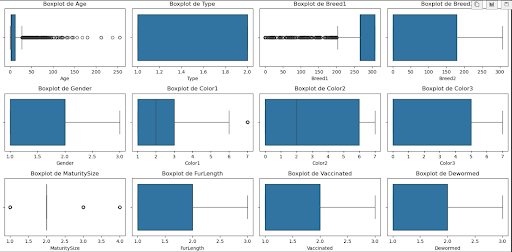
\includegraphics[width=0.65\textwidth]{boxplot_age_outliers.png}
    \caption{Boxplot illustrant les valeurs aberrantes de la variable Age}
    \label{fig:outliers_age}
\end{figure}






\subsection{Premier test : Régression logistique multiclasse}

Nous avons testé notre modèle à l’aide d’une régression logistique multiclasse afin de vérifier la cohérence des données et d’évaluer les performances de base. L’objectif était notamment de comparer les résultats obtenus à ceux du concours Kaggle, où une précision de 0{,}45 avait été atteinte.

Pour l’entraînement, nous avons utilisé les variables suivantes comme descripteurs : \texttt{Type}, \texttt{Age}, \texttt{Breed1}, \texttt{Breed2}, \texttt{Gender}, \texttt{Color1}, \texttt{Color2}, \texttt{Color3}, \texttt{MaturitySize}, \texttt{FurLength}, \texttt{Vaccinated}, \texttt{Dewormed}, \texttt{Sterilized}, \texttt{Health}, \texttt{Fee}, \texttt{VideoAmt} et \texttt{PhotoAmt}. La variable cible que nous cherchons à prédire est \texttt{AdoptionSpeed}, qui prend des valeurs entières de 0 à 4.

Le modèle a généré un \textbf{MSE de 2{,}2317}, avec un \textbf{biais de 1{,}9788} et une \textbf{variance de 0{,}2529}. La précision moyenne est d’environ \textbf{0{,}2699}. Ces résultats indiquent clairement un problème de \textbf{sous-apprentissage} : le biais est très élevé, ce qui suggère que le modèle n’arrive pas à capter la structure des données, et la précision est globalement très faible.

\begin{figure}[H]
    \centering
    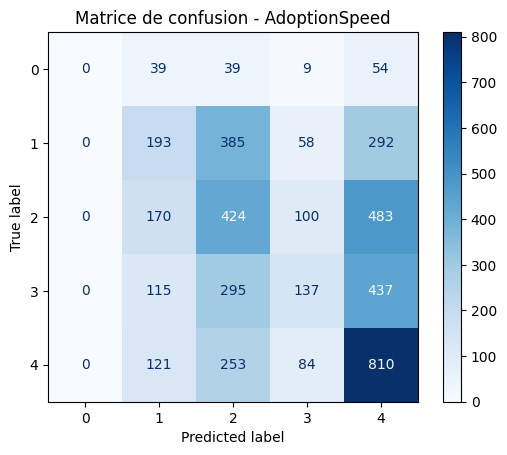
\includegraphics[width=0.75\textwidth]{matrice_confusion_logreg.png}
    \caption{Matrice de confusion obtenue avec la régression logistique}
    \label{fig:confusion_logreg}
\end{figure}

\begin{figure}[H]
    \centering
    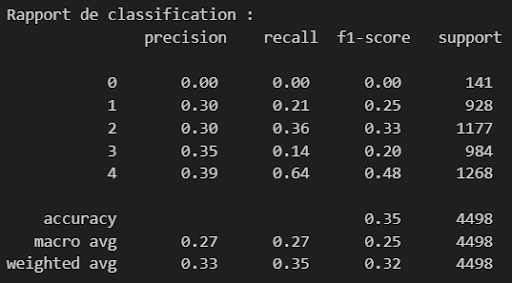
\includegraphics[width=0.75\textwidth]{classification_report_logreg.png}
    \caption{Rapport de classification - Régression logistique multiclasse}
    \label{fig:classification_logreg}
\end{figure}

L’analyse du rapport de classification et de la matrice de confusion confirme ces observations. On remarque notamment que la classe \textbf{0 n’est jamais prédite}, avec une précision et un rappel de \texttt{0.00}. Les autres classes sont également mal identifiées, avec des \textit{f1-scores} faibles et déséquilibrés. L’exactitude globale du modèle est d’environ \textbf{35 \%}, ce qui reste bien en dessous des attentes.

Un autre point préoccupant est le fort \textbf{déséquilibre dans la distribution des classes} au sein de la variable cible. La classe 0, par exemple, compte environ \textbf{six fois moins d’occurrences} que les autres, ce qui impacte fortement sa prédiction. Ce déséquilibre rend l’apprentissage difficile pour le modèle, qui a tendance à ignorer les classes minoritaires.

\subsection{Déséquilibre des classes}

La figure ci-dessous présente la répartition des animaux selon la variable \textit{AdoptionSpeed}, qui représente le délai d’adoption d’un animal. On observe une forte disparité entre les différentes classes. Plus de 4 000 animaux appartiennent à la classe 4 (non adoptés après plus de 100 jours), tandis que seulement 410 animaux relèvent de la classe 0 (adoptés le jour même).

Ce déséquilibre marqué peut poser un problème lors de l'entraînement de modèles de classification. En effet, un modèle pourrait être biaisé en faveur des classes majoritaires, au détriment des classes minoritaires qui sont pourtant d’un grand intérêt dans le contexte de prédiction. Par exemple, la classe 0, bien que peu représentée, fournit des informations précieuses sur les profils d’animaux très rapidement adoptés.

Ce constat justifie l’exploration de différentes stratégies de regroupement des classes ou de transformation de la cible, dans le but de construire un modèle plus robuste et plus pertinent.

\begin{figure}[H]
    \centering
    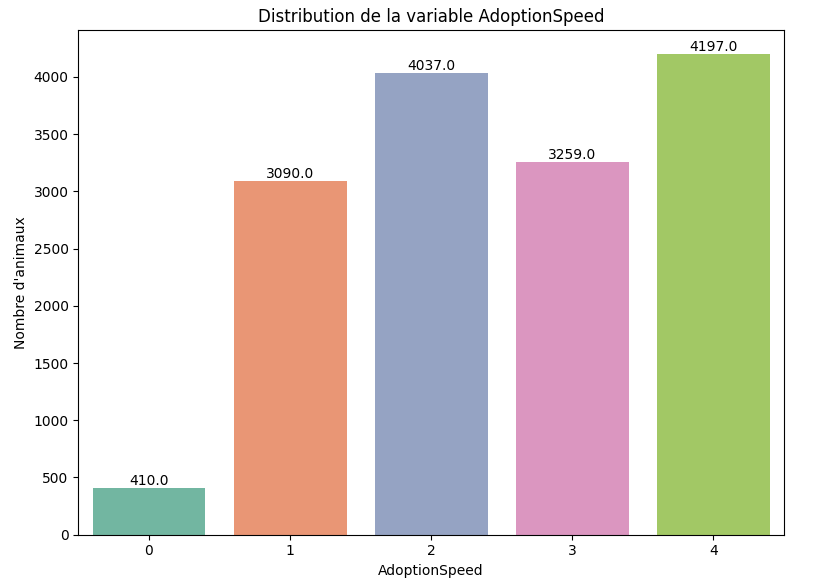
\includegraphics[width=0.7\textwidth]{adoption_speed_distribution.png}
    \caption{Répartition des animaux selon la vitesse d’adoption (AdoptionSpeed)}
    \label{fig:adoption_speed}
\end{figure}

\subsection{Utilisation de SMOTE pour l'équilibrage des classes}

Le dataset présente un déséquilibre marqué entre les classes de la variable \textit{AdoptionSpeed}, avec certaines classes nettement surreprésentées. Par exemple, la classe 0 comporte très peu d'échantillons par rapport aux classes 2 et 4. Ce déséquilibre a un impact négatif sur l’apprentissage du modèle, qui a tendance à privilégier les classes majoritaires au détriment des classes minoritaires.

Pour corriger cela, nous avons utilisé la technique SMOTE (\textit{Synthetic Minority Over-sampling Technique}), qui consiste à générer artificiellement de nouveaux exemples pour les classes minoritaires en interpolant les instances existantes.

\vspace{0.5em}
\noindent\textbf{Distribution des classes avant et après SMOTE}

La figure suivante illustre clairement l'effet de SMOTE. Avant son application, les classes sont inégalement réparties, avec une dominance des classes 2 et 4. Après SMOTE, toutes les classes comptent environ 2900 exemples, assurant un apprentissage plus équilibré du modèle.

\begin{figure}[H]
    \centering
    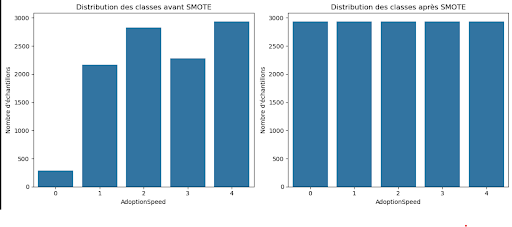
\includegraphics[width=0.8\textwidth]{distribution_smote.png}
    \caption{Distribution des classes avant (gauche) et après (droite) SMOTE}
    \label{fig:smote_distribution}
\end{figure}

\vspace{0.5em}
\noindent\textbf{Comparaison des performances avant et après SMOTE}

Les deux matrices de confusion ci-dessous comparent les performances du modèle avant et après l’équilibrage des classes. Sur le jeu de test original (non équilibré), le modèle montre un fort biais vers les classes fréquentes, comme 2 et 4. Après application de SMOTE, la répartition des prédictions devient plus homogène, traduisant une amélioration sur les classes minoritaires.

\begin{figure}[H]
    \centering
    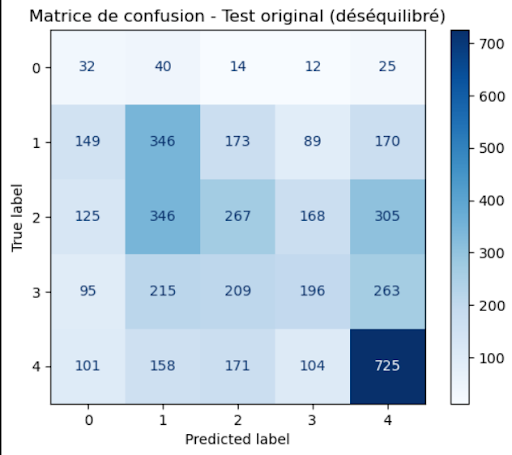
\includegraphics[width=0.45\textwidth]{matrice_confusion_avant_smote.png}
    \hfill
    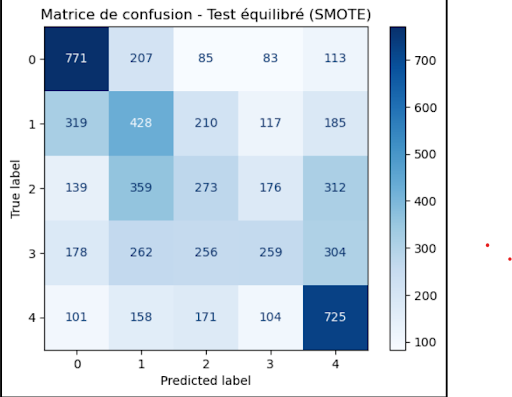
\includegraphics[width=0.45\textwidth]{matrice_confusion_apres_smote.png}
    \caption{Matrice de confusion avant (gauche) et après (droite) SMOTE}
    \label{fig:smote_matrices}
\end{figure}

\vspace{0.5em}
\noindent\textbf{Évolution des métriques globales}

\begin{figure}[H]
    \centering
    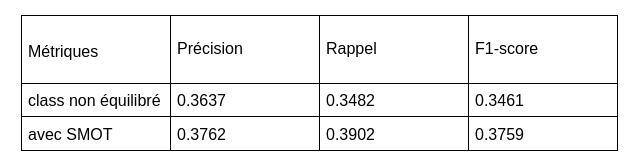
\includegraphics[width=0.6\textwidth]{resultats_smote_tableau.png}
    \caption{Résumé des performances avant et après SMOTE}
    \label{fig:smote_tableau}
\end{figure}

Les résultats montrent une amélioration modeste mais notable :
\begin{itemize}
    \item \textbf{Avant SMOTE} : précision = 0.3637, rappel = 0.3482, F1-score = 0.3461
    \item \textbf{Après SMOTE} : précision = 0.3762, rappel = 0.3902, F1-score = 0.3759
\end{itemize}

Ces résultats confirment l’intérêt de SMOTE pour améliorer la reconnaissance des classes rares, tout en limitant l’effet de surapprentissage.


\subsection{Amélioration par duplication de la classe 0}

Vérifions maintenant si l’absence de prédiction pour la classe \texttt{0} est due à son extrême rareté par rapport aux autres classes. Pour cela, nous avons artificiellement augmenté les occurrences de cette classe en multipliant ses \textbf{410 lignes par 7}, afin d’obtenir environ \textbf{3090 lignes}, ce qui permet d’équilibrer un peu plus les proportions avec les autres classes.

Nous avons ensuite réentraîné notre modèle de régression logistique multiclasse avec ce nouvel ensemble de données. Les résultats obtenus sont les suivants :
\begin{itemize}
    \item \textbf{MSE :} 3.6941
    \item \textbf{Biais :} 3.3316
    \item \textbf{Variance :} 0.3626
    \item \textbf{Précision globale :} 0.2893
\end{itemize}

La précision a donc légèrement augmenté (\textbf{+2 points}), mais cela ne s’est pas traduit par une réelle amélioration du modèle. En réalité, le nombre d’erreurs a augmenté, ce qui montre que le modèle reste peu performant.

\begin{figure}[H]
    \centering
    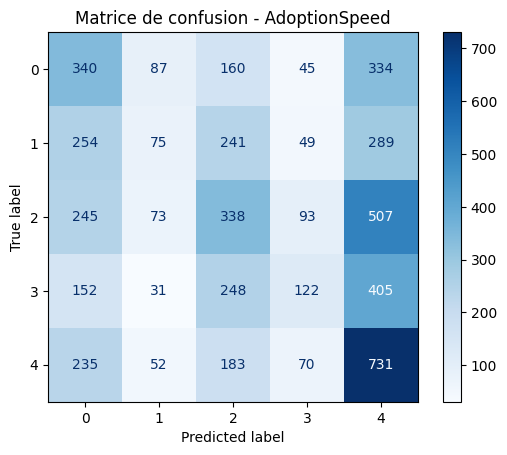
\includegraphics[width=0.75\textwidth]{confusion_logreg_multiplication_classe0.png}
    \caption{Matrice de confusion après duplication de la classe 0}
    \label{fig:confusion_logreg_duplicated}
\end{figure}

\begin{figure}[H]
    \centering
    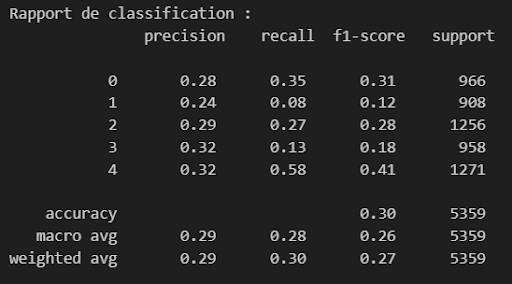
\includegraphics[width=0.75\textwidth]{classification_report_logreg_multiplication.png}
    \caption{Rapport de classification après duplication de la classe 0}
    \label{fig:report_logreg_duplicated}
\end{figure}

Malgré tout, on observe une \textbf{amélioration de la précision pour la classe 0}, qui est désormais mieux prise en compte. Cependant, cette classe est \textbf{souvent confondue avec la classe 4}, ainsi qu’avec d’autres classes, ce qui limite l’efficacité de la prédiction.

\medskip

En conclusion, le modèle est toujours en situation de \textbf{sous-apprentissage}. Il souffrait clairement du manque d’occurrences pour la classe 0, mais il est aussi handicapé par une forte similarité entre les variables descriptives. Cette proximité rend difficile la discrimination entre les différentes classes. Pour améliorer cela, il serait nécessaire d’ajouter de nouvelles variables plus discriminantes, que nous ne possédons pas actuellement.


\bigskip

Au-delà des performances quantitatives obtenues via les modèles supervisés, il est essentiel de mieux comprendre la structure intrinsèque des données. C’est dans cette optique que nous avons mené des analyses exploratoires complémentaires, telles que le clustering non supervisé et l’Analyse des Correspondances Multiples (ACM), afin d’identifier les tendances cachées dans la distribution des classes et de détecter d’éventuels regroupements naturels entre les observations.

\subsection{Analyse des tendances globales des variables catégorielles}

Les histogrammes ci-dessous illustrent la répartition des variables catégoriques \texttt{Type}, \texttt{Gender}, \texttt{MaturitySize}, \texttt{FurLength}, \texttt{Vaccinated}, \texttt{Dewormed} et \texttt{Sterilized} selon les différentes classes de la variable \texttt{AdoptionSpeed}.

On observe une tendance générale similaire entre les classes pour toutes ces variables. Pour \texttt{Type}, les catégories \textit{Cat} (bleu) et \textit{Dog} (orange) sont globalement équilibrées dans chaque classe (de 0 à 4). En ce qui concerne \texttt{Gender}, les animaux de genre \textit{Male} (bleu) et \textit{Female} (orange) sont majoritaires, tandis que la catégorie \textit{Not Specified} (vert) reste marginale.

Pour la variable \texttt{MaturitySize}, la taille \textit{Medium} (bleu) domine largement, suivie de \textit{Small} (orange), tandis que les tailles \textit{Large} (vert) et \textit{Extra Large} (rouge) sont peu représentées. Une tendance similaire est observée pour \texttt{FurLength}, où les longueurs \textit{Short} (orange) et \textit{Medium} (bleu) prédominent, avec une faible occurrence de \textit{Long} (vert).

Enfin, pour les variables \texttt{Vaccinated}, \texttt{Dewormed} et \texttt{Sterilized}, les réponses \textit{No} (orange) et \textit{Yes} (vert) sont les plus représentées, tandis que \textit{Not Sure} (bleu) est moins fréquente.

Cette homogénéité des répartitions rend difficile l’identification de variables discriminantes permettant de bien séparer les classes de \texttt{AdoptionSpeed}. Aucune des variables observées ne présente une tendance distincte ou marquée entre les classes, ce qui peut expliquer la difficulté rencontrée par les modèles pour prédire efficacement la vitesse d’adoption.

\begin{figure}[H]
    \centering
    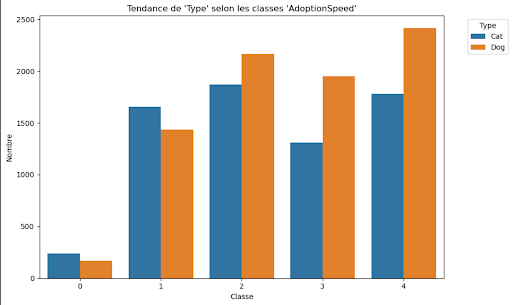
\includegraphics[width=0.75\textwidth]{type_adoption_trend.png}
    \caption{Tendance de la variable \texttt{Type} selon les classes d'\texttt{AdoptionSpeed}}
    \label{fig:type_trend}
\end{figure}

\begin{figure}[H]
    \centering
    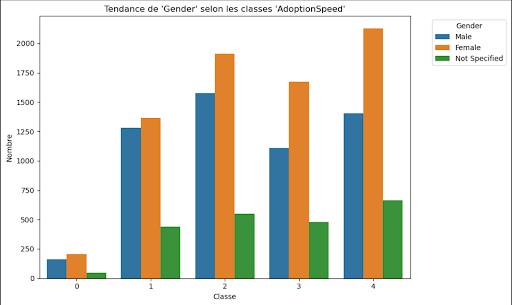
\includegraphics[width=0.75\textwidth]{gender_adoption_trend.png}
    \caption{Tendance de la variable \texttt{Gender} selon les classes d'\texttt{AdoptionSpeed}}
    \label{fig:gender_trend}
\end{figure}

\begin{figure}[H]
    \centering
    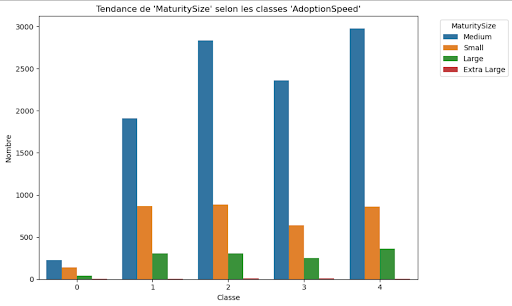
\includegraphics[width=0.75\textwidth]{maturitysize_adoption_trend.png}
    \caption{Tendance de la variable \texttt{MaturitySize} selon les classes d'\texttt{AdoptionSpeed}}
    \label{fig:maturitysize_trend}
\end{figure}

\begin{figure}[H]
    \centering
    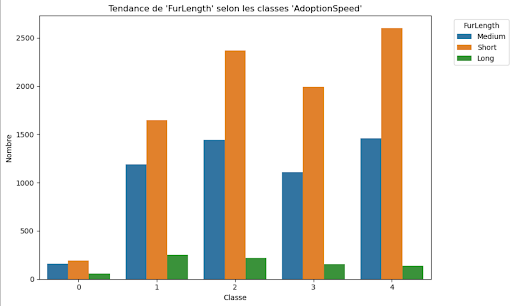
\includegraphics[width=0.75\textwidth]{furlength_adoption_trend.png}
    \caption{Tendance de la variable \texttt{FurLength} selon les classes d'\texttt{AdoptionSpeed}}
    \label{fig:furlength_trend}
\end{figure}

\begin{figure}[H]
    \centering
    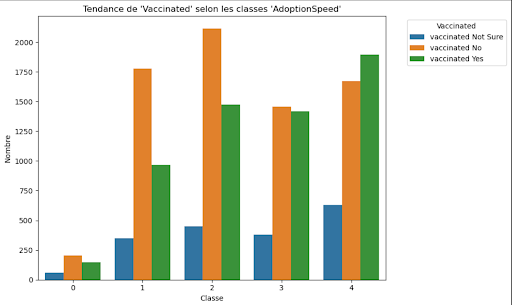
\includegraphics[width=0.75\textwidth]{vaccinated_adoption_trend.png}
    \caption{Tendance de la variable \texttt{Vaccinated} selon les classes d'\texttt{AdoptionSpeed}}
    \label{fig:vaccinated_trend}
\end{figure}

\begin{figure}[H]
    \centering
    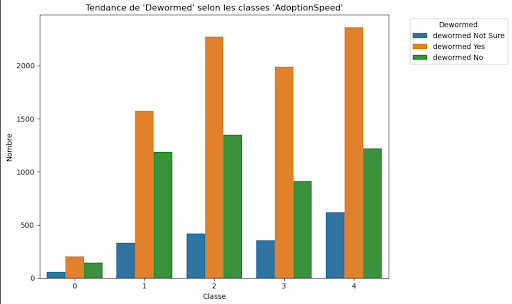
\includegraphics[width=0.75\textwidth]{dewormed_adoption_trend.png}
    \caption{Tendance de la variable \texttt{Dewormed} selon les classes d'\texttt{AdoptionSpeed}}
    \label{fig:dewormed_trend}
\end{figure}

\begin{figure}[H]
    \centering
    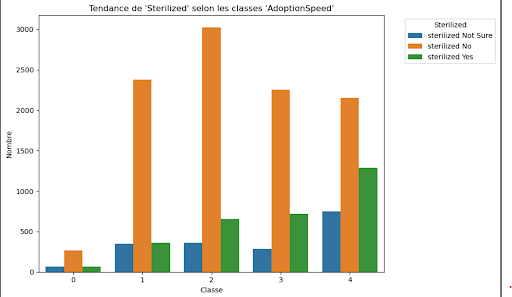
\includegraphics[width=0.75\textwidth]{sterilized_adoption_trend.png}
    \caption{Tendance de la variable \texttt{Sterilized} selon les classes d'\texttt{AdoptionSpeed} (graphe 1)}
    \label{fig:sterilized_trend_1}
\end{figure}

\begin{figure}[H]
    \centering
    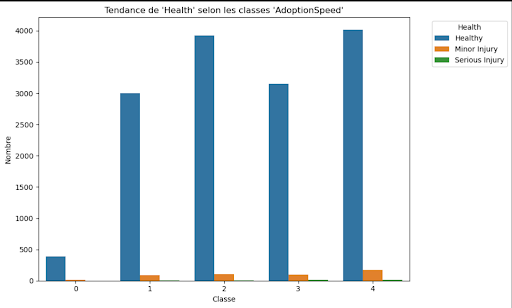
\includegraphics[width=0.75\textwidth]{health_adoption_trend.png}
    \caption{Tendance de la variable \texttt{Health} selon les classes d'\texttt{AdoptionSpeed}}
    \label{fig:health_trend}
\end{figure}

\subsection{Analyse en Composantes Multiples (ACM)}

Afin de mieux comprendre les relations entre les variables qualitatives du jeu de données, une Analyse en Composantes Multiples (ACM) a été réalisée. Cette méthode permet de visualiser la structure des données catégorielles et d’identifier d’éventuelles associations entre les modalités des différentes variables.

\begin{figure}[H]
    \centering
    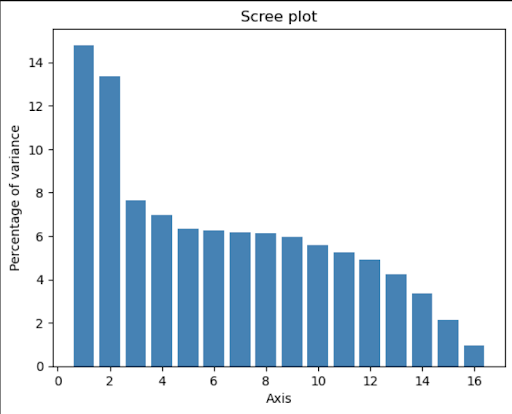
\includegraphics[width=0.7\textwidth]{acm_variance.png}
    \caption{Répartition de la variance expliquée par chaque axe de l'ACM (Scree plot)}
    \label{fig:acm_scree}
\end{figure}

Le premier graphe (Figure~\ref{fig:acm_scree}) montre la répartition de la variance expliquée par chaque axe. On observe que la première dimension (Dim 1) explique 14,8\% de la variance totale, et la deuxième (Dim 2) 13,35\%. Ensemble, ces deux axes capturent environ 28\% de l'information globale, ce qui est suffisant pour une visualisation initiale. La décroissance progressive de la variance suggère que les premières dimensions concentrent l’essentiel des variations dans les données.

\begin{figure}[H]
    \centering
    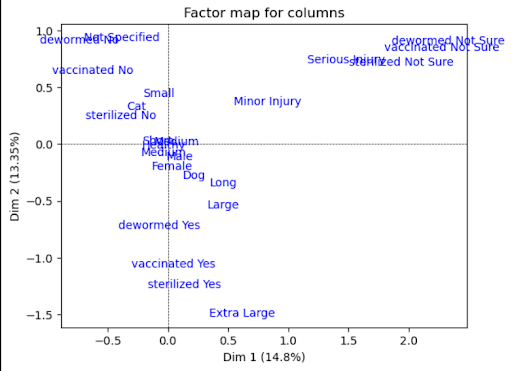
\includegraphics[width=0.8\textwidth]{acm_factor_map.png}
    \caption{Carte factorielle des modalités (ACM)}
    \label{fig:acm_modalites}
\end{figure}

La carte factorielle des modalités (Figure~\ref{fig:acm_modalites}) illustre les liens entre les modalités des variables catégorielles. Certaines associations apparaissent clairement :

\begin{itemize}
    \item Les modalités \textit{vaccinated YES}, \textit{dewormed YES}, et \textit{sterilized YES} sont regroupées dans le quadrant inférieur gauche, montrant une forte corrélation entre ces traitements sanitaires.
    \item Les modalités opposées \textit{vaccinated NO}, \textit{dewormed NO}, et \textit{sterilized NO} apparaissent ensemble dans le quadrant supérieur gauche.
    \item Un groupe particulier est formé par les modalités \textit{vaccinated NOT SURE}, \textit{dewormed NOT SURE}, et \textit{sterilized NOT SURE}, dans le quadrant supérieur droit.
    \item Les modalités liées au genre (\textit{Male} et \textit{Female}) et à la taille (\textit{Medium}, \textit{Small}, \textit{Large}, \textit{Extra Large}) sont proches de l’origine. Cela indique une faible contribution discriminante sur les deux premiers axes.
\end{itemize}

Ces observations confirment les résultats des histogrammes présentés précédemment : les tendances sont globalement homogènes entre les classes d’\textit{AdoptionSpeed}, et aucune variable catégorielle n’émerge clairement comme discriminante. Cela illustre la complexité du problème de classification et justifie le recours à des regroupements de classes pour faciliter l’apprentissage.



\subsection{Analyse des clusters : vers une réduction du nombre de classes}

Dans le cadre de notre étude, une analyse de clustering non supervisé a été réalisée afin d’évaluer la cohérence des classes d’adoption existantes dans les données. Pour cela, nous avons utilisé l’algorithme \textit{K-Means}, appliqué aux données préalablement standardisées. Une réduction de dimension par \textbf{ACM}  a été effectuée pour projeter les observations sur deux axes principaux, notés \textit{Composante principale 1} et \textit{Composante principale 2}. Ces deux axes représentent les directions dans lesquelles les données varient le plus, ce qui permet de mieux visualiser la structure des groupes.

Deux configurations ont été testées : un clustering en \textbf{5 groupes} et un clustering en \textbf{2 groupes}.

\begin{figure}[H]
    \centering
    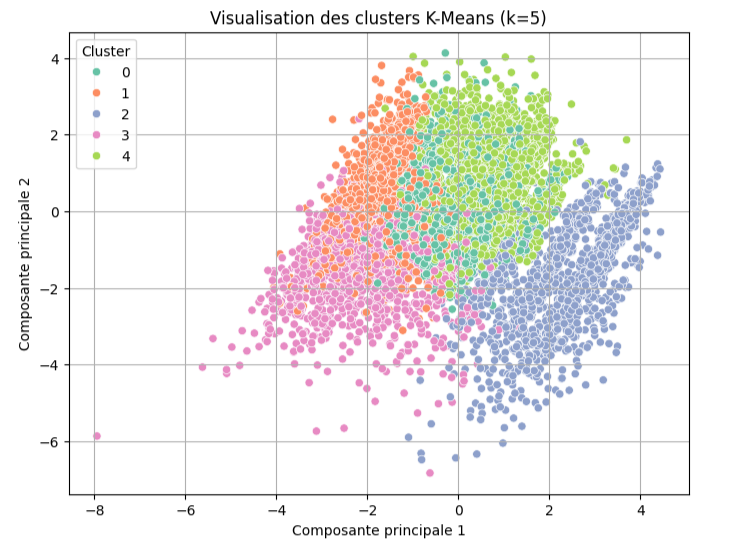
\includegraphics[width=0.7\textwidth]{graph_kmeans_5.png}
    \caption{Clustering KMeans avec $k=5$}
    \label{fig:kmeans_5}
\end{figure}

\begin{figure}[H]
    \centering
    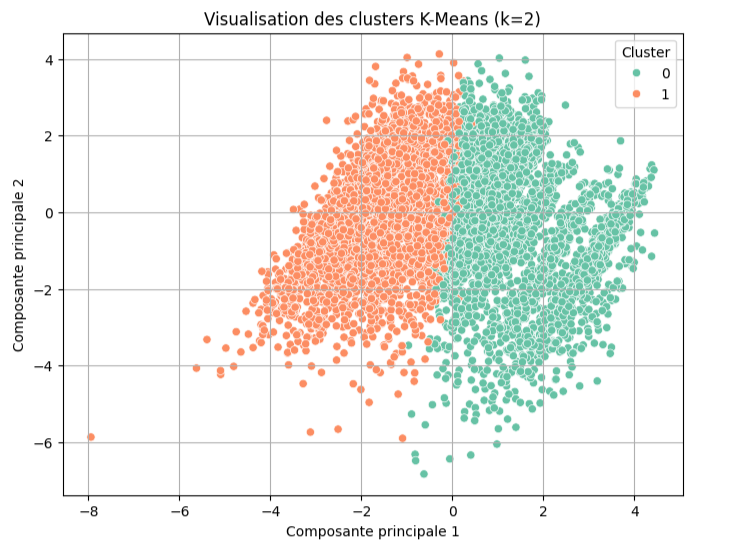
\includegraphics[width=0.7\textwidth]{graph_kmeans_2.png}
    \caption{Clustering KMeans avec $k=2$}
    \label{fig:kmeans_2}
\end{figure}

Le graphe avec $k=5$ montre un chevauchement important entre les groupes, ce qui suggère que la distinction entre les 5 catégories d’adoption n’est pas clairement définie dans l’espace des données. À l’inverse, la représentation avec $k=2$ montre des groupes bien séparés, suggérant qu’un découpage en \textbf{deux catégories globales} serait plus pertinent. Cela renforce l’idée que le problème de prédiction est sans doute mal posé avec 5 classes trop proches ou arbitraires, et qu’un regroupement permettrait une classification plus robuste.

\subsection{Comparaison de regroupements de classes avec Random Forest}

Afin d’optimiser la prédiction de la vitesse d’adoption des animaux, nous avons exploré deux regroupements binaires alternatifs à la classification initiale en 5 classes. L’objectif est de simplifier le problème tout en conservant une interprétabilité pertinente.

Les deux combinaisons testées sont :
\begin{itemize}
    \item \textbf{Combinaison 1} : \texttt{[0,1,2]} vs \texttt{[3,4]} — où \texttt{0} représente une adoption rapide ou modérée, et \texttt{1} une adoption lente ou non adoption.
    \item \textbf{Combinaison 2} : \texttt{[1,2]} vs \texttt{[3,4]} — où la classe \texttt{0} (adoption le jour même) est exclue.
\end{itemize}

Ces regroupements ont été évalués à l’aide d’un modèle \textbf{Random Forest} avec une validation croisée à 5 plis, et en mesurant plusieurs métriques : \textit{accuracy}, \textit{precision}, \textit{recall}, \textit{F1-score}, mais aussi le biais, la variance et l’erreur quadratique moyenne (MSE).

\vspace{0.3cm}
\begin{table}[h]
\centering
\begin{tabular}{|l|c|c|c|c|c|c|c|c|}
\hline
\textbf{Regroupement} & \textbf{Accuracy} & \textbf{Précision} & \textbf{Recall} & \textbf{F1-score} & \textbf{MSE} & \textbf{Biais} & \textbf{Variance} \\
\hline
\texttt{[0,1,2]} vs \texttt{[3,4]} & 62.7\% & 62.7\% & 62.7\% & 62.7\% & 0.376 & 0.274 & 0.101  \\
\texttt{[1,2]} vs \texttt{[3,4]}   & 61.4\% & 61.5\% & 61.4\% & 61.5\% & 0.385 & 0.284 & 0.101  \\
\hline
\end{tabular}
\caption{Comparaison des performances entre deux regroupements de classes avec Random Forest}
\end{table}

\noindent
On observe que la première combinaison \texttt{[0,1,2]} vs \texttt{[3,4]} donne de meilleures performances globales, avec un F1-score de \textbf{62.7\%}, une \textit{erreur quadratique moyenne (MSE)} plus faible, ainsi qu’un \textit{biais} plus bas. Cela suggère qu'inclure la classe 0 (adoption immédiate) dans les cas d’adoption rapide/modérée améliore la robustesse du modèle.

Ce résultat conforte l'idée que le reclassement judicieux de la variable cible peut améliorer les performances prédictives, tout en gardant du sens dans l'interprétation métier.
\subsubsection{Optimisation des performances avec GridSearchCV}

Afin d'améliorer les performances du modèle Random Forest, une recherche d'hyperparamètres a été réalisée à l’aide de \texttt{GridSearchCV}, en explorant plusieurs combinaisons de paramètres tels que \texttt{max\_depth}, \texttt{n\_estimators}, \texttt{min\_samples\_split}, \texttt{min\_samples\_leaf}, et \texttt{max\_features}. Deux regroupements de classes ont été testés : \textbf{(0,1,2) vs (3,4)} et \textbf{(1,2) vs (3,4)}.

Les meilleurs paramètres trouvés par GridSearch pour les deux cas sont :
\begin{itemize}
    \item \texttt{max\_depth=10}, \texttt{n\_estimators=200}, \texttt{min\_samples\_split=5}, \texttt{min\_samples\_leaf=2}, \texttt{max\_features='sqrt'}
\end{itemize}

\paragraph{Résultats pour le regroupement (0,1,2) vs (3,4) :}
\begin{itemize}
    \item Accuracy : 65.07\%
    \item Précision : 65.09\%
    \item Rappel : 65.07\%
    \item F1-score : 65.05\%
    \item MSE : 0.3553
    \item Biais : 0.2948
    \item Variance : 0.0605
    \item Moyenne de validation croisée : 64.6\%
\end{itemize}

\paragraph{Résultats pour le regroupement (1,2) vs (3,4) :}
\begin{itemize}
    \item Accuracy : 65.07\%
    \item Précision : 65.09\%
    \item Rappel : 65.07\%
    \item F1-score : 65.05\%
    \item MSE : 0.3553
    \item Biais : 0.2948
    \item Variance : 0.0605
    \item Moyenne de validation croisée : 64.6\%
\end{itemize}



Les deux regroupements donnent des résultats quasiment identiques après optimisation, confirmant la robustesse du modèle Random Forest. Toutefois, on remarque que le gain en performance reste marginal après optimisation, suggérant qu’une approche plus fine comme l’analyse de nouvelles variables ou le test d’autres algorithmes pourrait être plus prometteuse pour améliorer les performances globales.

\subsection{Comparaison des résultats avec CatBoost sur différents regroupements de classes}

Pour approfondir l’analyse des regroupements de classes, nous avons évalué les performances du modèle \textbf{CatBoost} sur deux combinaisons binaires : 
\begin{itemize}
    \item Regroupement des classes \textbf{(0+1+2)} contre \textbf{(3+4)}.
    \item Regroupement des classes \textbf{(1+2)} contre \textbf{(3+4)}.
\end{itemize}

\paragraph{1. Regroupement (0+1+2) vs (3+4) :}

Dans cette configuration, le modèle CatBoost a montré des résultats globalement satisfaisants. Le \textbf{MSE est de 0.3498}, accompagné d’un \textbf{biais de 0.2741} et d’une \textbf{variance de 0.0758}. La précision globale atteint \textbf{66.16\%}, tout comme le rappel et le f1-score, ce qui montre une bonne stabilité du modèle et une performance équilibrée entre les deux classes. La matrice de confusion indique que la majorité des exemples sont bien prédits, avec une légère confusion entre les classes.

\begin{figure}[H]
    \centering
    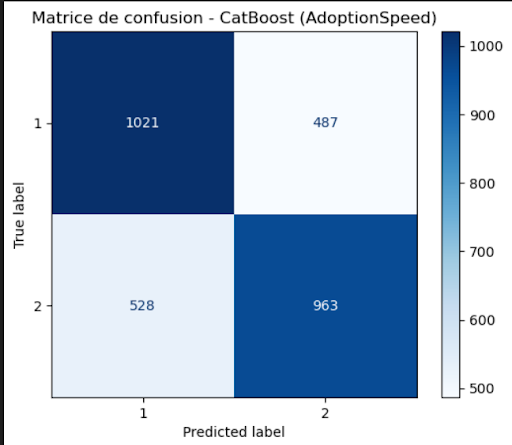
\includegraphics[width=0.65\textwidth]{catboost_012_vs_34_confusion.png}
    \caption{Matrice de confusion - CatBoost (regroupement 0+1+2 vs 3+4)}
    \label{fig:catboost012_conf}
\end{figure}

\begin{figure}[H]
    \centering
    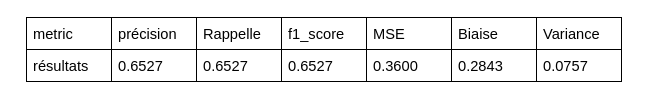
\includegraphics[width=0.55\textwidth]{catboost_012_vs_34_scores.png}
    \caption{Tableau des scores - CatBoost (regroupement 0+1+2 vs 3+4)}
    \label{fig:catboost012_scores}
\end{figure}

\paragraph{2. Regroupement (1+2) vs (3+4) :}

Ce deuxième regroupement a également été testé afin de voir si l'exclusion de la classe 0 (rare) pouvait améliorer la performance. Le modèle atteint une \textbf{précision de 65.27\%}, un rappel et un f1-score identiques, ainsi qu’un \textbf{MSE de 0.3600}, un biais de 0.2843 et une variance de 0.0757. Les résultats sont légèrement inférieurs à ceux du regroupement précédent, ce qui indique que l'exclusion de la classe 0 n’a pas permis de gains significatifs.

\begin{figure}[H]
    \centering
    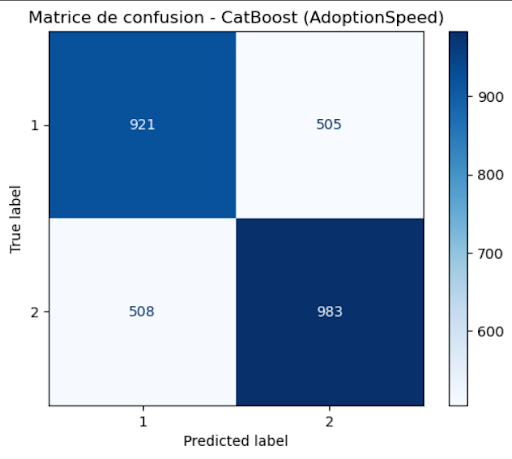
\includegraphics[width=0.65\textwidth]{catboost_12_vs_34_confusion.png}
    \caption{Matrice de confusion - CatBoost (regroupement 1+2 vs 3+4)}
    \label{fig:catboost12_conf}
\end{figure}

\begin{figure}[H]
    \centering
    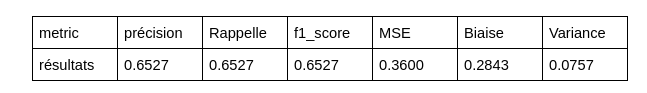
\includegraphics[width=0.55\textwidth]{catboost_12_vs_34_scores.png}
    \caption{Tableau des scores - CatBoost (regroupement 1+2 vs 3+4)}
    \label{fig:catboost12_scores}
\end{figure}

\paragraph{Conclusion :} Ces résultats montrent que CatBoost parvient à modéliser correctement les regroupements binaires, avec une stabilité des prédictions (variance faible) et un compromis intéressant entre biais et variance. Le regroupement \textbf{(0+1+2) vs (3+4)} donne des performances légèrement supérieures.

\subsection{Comparaison des combinaisons avec Gradient Boosting}

\subsubsection{Entraînement du modèle Gradient Boosting — combinaison (0,1,2) vs (3,4)}

Pour améliorer la performance du modèle, nous avons fusionné les classes 0, 1 et 2 en une classe 0, et les classes 3 et 4 en une classe 1. Cette transformation vise à simplifier le problème en une tâche de classification binaire mieux équilibrée.

Les résultats obtenus montrent un \textbf{MSE} de \textbf{0.3606}, un biais modéré de \textbf{0.2980}, et une variance faible de \textbf{0.0626}, indiquant une bonne stabilité des prédictions et une capacité de généralisation convenable. La précision moyenne en validation croisée (macro) atteint \textbf{64.83 \%} et l'\textbf{accuracy globale} est de \textbf{64.55 \%}, des valeurs satisfaisantes bien qu'améliorables.

\begin{figure}[H]
    \centering
    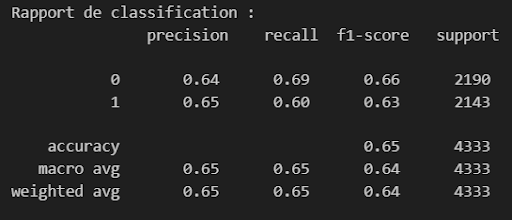
\includegraphics[width=0.8\textwidth]{classification_report_gb_012_vs_34.png}
    \caption{Rapport de classification — Gradient Boosting (0,1,2) vs (3,4)}
    \label{fig:gb_report_012_34}
\end{figure}

Le rapport de classification révèle que pour la classe 0, la précision est de 0.64, le rappel de 0.69 et le f1-score de 0.66, tandis que pour la classe 1, la précision est légèrement meilleure à 0.65, mais avec un rappel plus faible de 0.60, donnant un f1-score de 0.63. Cela montre que la classe 0 est mieux reconnue, mais la classe 1 reste plus difficile à identifier correctement.

\begin{figure}[H]
    \centering
    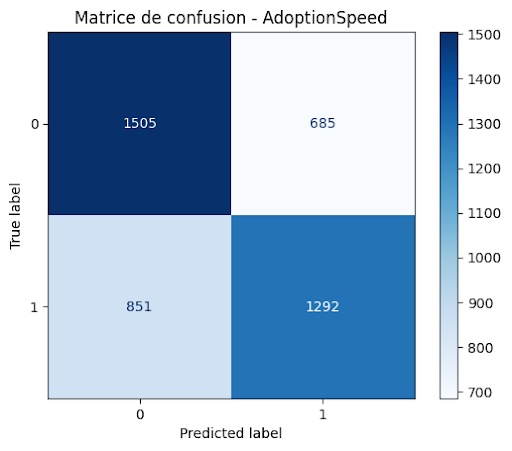
\includegraphics[width=0.75\textwidth]{confusion_matrix_gb_012_vs_34.png}
    \caption{Matrice de confusion — Gradient Boosting (0,1,2) vs (3,4)}
    \label{fig:gb_confusion_012_34}
\end{figure}

La matrice de confusion indique que \textbf{1505 exemples de la classe 0} et \textbf{1292 exemples de la classe 1} sont bien prédits, mais respectivement \textbf{685 exemples de la classe 0} et \textbf{851 de la classe 1} sont mal classés. Globalement, le \textbf{recall} est de \textbf{60.29 \%}, et la \textbf{précision globale} atteint \textbf{65.35 \%}, soulignant une confiance correcte dans les prédictions, bien qu'elle se fasse au détriment du rappel.

\subsubsection{Entraînement du modèle Gradient Boosting — combinaison (1,2) vs (3,4)}

Dans cette seconde approche, la classe 0, très minoritaire, a été supprimée pour réduire le déséquilibre. Les classes 1 et 2 ont été regroupées sous l’étiquette 0, et les classes 3 et 4 sous l’étiquette 1, transformant ainsi le problème en une classification binaire plus équilibrée.

Cette approche a conduit à des résultats prometteurs : le \textbf{score de précision macro moyen} atteint \textbf{0.6516}, indiquant une nette amélioration par rapport aux modèles multiclasse précédents. Le \textbf{MSE}, à \textbf{0.3605}, montre une stabilité accrue des prédictions, tandis que le \textbf{biais} (\textbf{0.2994}) reste modéré et la \textbf{variance} faible (\textbf{0.0611}), signe d’une bonne généralisation sans surajustement.

\begin{figure}[H]
    \centering
    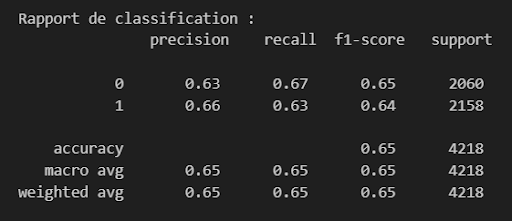
\includegraphics[width=0.8\textwidth]{classification_report_gb_12_vs_34.png}
    \caption{Rapport de classification — Gradient Boosting (1,2) vs (3,4)}
    \label{fig:gb_report_12_34}
\end{figure}

Le rapport de classification reflète un bon équilibre entre les classes : la classe 0 atteint une précision de 0.63 et un rappel de 0.67, tandis que la classe 1 affiche une précision de 0.66 et un rappel de 0.63, avec des f1-scores similaires (\textbf{0.64}-\textbf{0.65}), prouvant l’absence de biais en faveur d’une classe.

\begin{figure}[H]
    \centering
    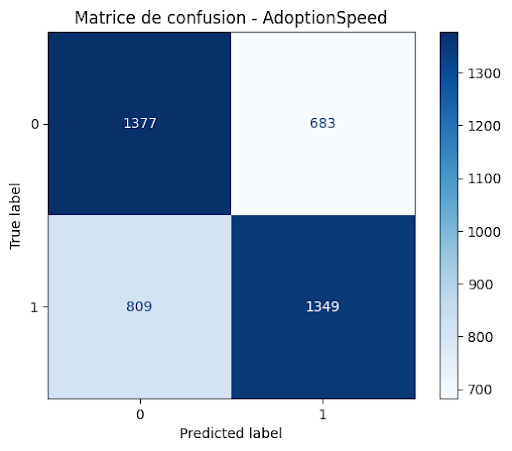
\includegraphics[width=0.75\textwidth]{confusion_matrix_gb_12_vs_34.png}
    \caption{Matrice de confusion — Gradient Boosting (1,2) vs (3,4)}
    \label{fig:gb_confusion_12_34}
\end{figure}

La matrice de confusion montre une classification correcte pour la majorité des exemples : \textbf{1377 exemples sur 2060} pour la classe 0 et \textbf{1349 sur 2158} pour la classe 1. Enfin, le modèle atteint une \textbf{précision globale de 66.39 \%}, un \textbf{rappel global de 62.51 \%} et une \textbf{accuracy de 64.63 \%}.
\subsubsection{Comparaison des deux combinaisons avec Gradient Boosting}

Afin d’identifier la meilleure manière de regrouper les classes d’adoption, nous avons comparé deux approches de fusion :
\begin{itemize}
    \item \textbf{Fusion (0,1,2)} contre \textbf{(3,4)}
    \item \textbf{Fusion (1,2)} contre \textbf{(3,4)}
\end{itemize}

Les résultats obtenus à l’issue des expérimentations avec l’algorithme Gradient Boosting sont résumés dans le tableau ci-dessous :

\begin{figure}[H]
    \centering
    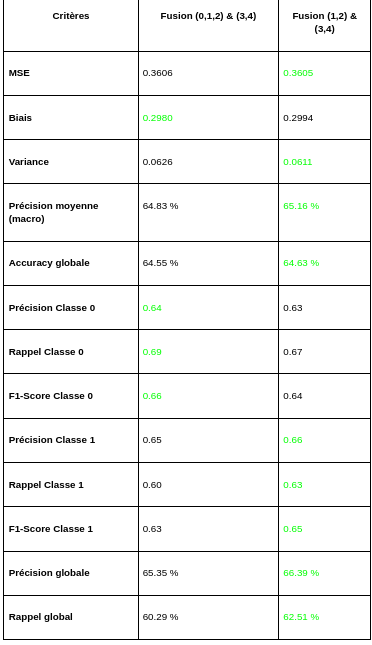
\includegraphics[width=0.65\textwidth]{capture_fusion_gb_tableau.png}
    \caption{Comparaison des performances entre les deux fusions de classes}
    \label{fig:comparaison_fusion_gradient_boosting}
\end{figure}

La \textbf{fusion (0,1,2) \& (3,4)} présente un biais légèrement inférieur (0.2980 contre 0.2994), ce qui pourrait indiquer un risque légèrement réduit de sous-apprentissage. Cependant, la variance est un peu plus élevée (0.0626 contre 0.0611), suggérant une stabilité des prédictions légèrement moindre et un risque un peu plus élevé de sur-apprentissage par rapport à l'approche \textbf{(1,2) \& (3,4)}.

En termes de prédictions, la \textbf{fusion (1,2) \& (3,4)} offre un équilibre supérieur entre précision et rappel pour les deux classes, avec des f1-scores légèrement meilleurs et une précision globale plus élevée (66.39 \% contre 65.35 \%), ce qui montre une performance générale légèrement meilleure.

\textbf{Conclusion :} La fusion \textbf{(1,2) \& (3,4)} s’avère être la meilleure option, offrant une meilleure généralisation et un équilibre supérieur entre le sous-apprentissage et le sur-apprentissage.

\subsection{Ajout des sentiments textuels dans le Gradient Boosting}

Après avoir fusionné les classes \textbf{1 et 2} en une classe \textbf{0}, et les classes \textbf{3 et 4} en une classe \textbf{1}, nous avons enrichi notre modèle en y intégrant des variables dérivées de l’analyse textuelle des descriptions des animaux. Ces nouvelles variables correspondent aux scores de sentiment \textit{positif}, \textit{négatif} et \textit{neutre} extraits des textes descriptifs.

Le modèle Gradient Boosting, réentraîné avec ces nouvelles variables, a obtenu les performances suivantes :
\begin{itemize}
    \item \textbf{Précision moyenne (macro)} en validation croisée : 64.71\,\%
    \item \textbf{Accuracy globale} : 64.25\,\%
    \item \textbf{MSE} : 0.3627
    \item \textbf{Biais} : 0.2894
    \item \textbf{Variance} : 0.0733
\end{itemize}

Ces résultats témoignent d'une \textbf{stabilité générale du modèle}, avec une faible variance, signe d'un surapprentissage limité.

\begin{figure}[H]
    \centering
    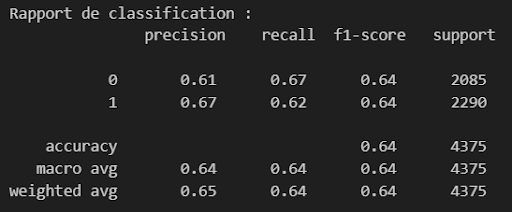
\includegraphics[width=0.7\textwidth]{image-rapport-classification.png}
    \caption{Rapport de classification avec ajout des variables de sentiment}
    \label{fig:rapport_sentiment}
\end{figure}

Sur le plan des classes :
\begin{itemize}
    \item \textbf{Classe 0} : Précision = 0.61, Rappel = 0.67, F1-score = 0.64
    \item \textbf{Classe 1} : Précision = 0.67, Rappel = 0.62, F1-score = 0.64
\end{itemize}

Ces scores sont relativement équilibrés, montrant une reconnaissance modérée mais stable des deux classes.

\begin{figure}[H]
    \centering
    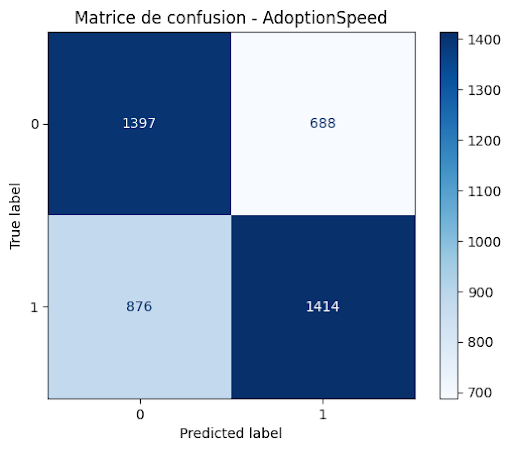
\includegraphics[width=0.7\textwidth]{image-matrice-confusion.png}
    \caption{Matrice de confusion avec ajout des variables de sentiment}
    \label{fig:matrice_sentiment}
\end{figure}

La matrice de confusion met en évidence des erreurs notables :
\begin{itemize}
    \item \textbf{688} exemples de la classe 0 sont prédit comme appartenant à la classe 1
    \item \textbf{876} exemples de la classe 1 sont mal classés en classe 0
\end{itemize}

Malgré ces confusions importantes, la \textbf{précision globale augmente légèrement à 67.27\,\%}, ce qui suggère que les variables liées au \textit{sentiment} apportent un signal pertinent, bien que l'amélioration reste modeste.


\subsection{Optimisation du Gradient Boosting avec les sentiments (GridSearchCV)}

Après optimisation des hyperparamètres du modèle Gradient Boosting à l’aide de \texttt{GridSearchCV}, les meilleurs paramètres retenus sont :
\begin{itemize}
    \item \texttt{learning\_rate} = 0.01
    \item \texttt{max\_depth} = 7
    \item \texttt{n\_estimators} = 300
    \item \texttt{subsample} = 0.8
\end{itemize}

L’objectif était d’améliorer les performances du modèle enrichi par les variables de sentiment, tout en conservant une bonne capacité de généralisation. 

Les résultats obtenus après entraînement avec ces paramètres sont :
\begin{itemize}
    \item \textbf{Accuracy} : 64.00\,\%
    \item \textbf{MSE} : 0.3607
    \item \textbf{Biais} : 0.2875
    \item \textbf{Variance} : 0.0732
\end{itemize}

Ces métriques traduisent un bon équilibre entre biais et variance, sans réel gain par rapport au modèle précédent sans optimisation.

\begin{figure}[H]
    \centering
    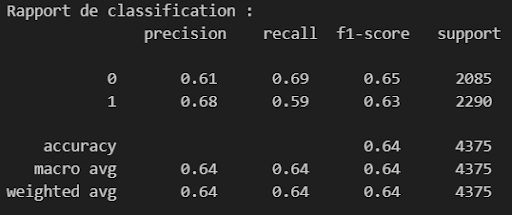
\includegraphics[width=0.7\textwidth]{classification_sentiment_gridsearch.png}
    \caption{Rapport de classification -- Gradient Boosting avec sentiments (optimisé)}
    \label{fig:classification_sentiment_gridsearch}
\end{figure}

D’après le rapport de classification :
\begin{itemize}
    \item \textbf{Classe 0} : Précision = 0.61, Rappel = 0.69, F1-score = 0.65
    \item \textbf{Classe 1} : Précision = 0.68, Rappel = 0.59, F1-score = 0.63
\end{itemize}

On observe une répartition relativement équilibrée entre les deux classes, bien que la classe 1 présente un rappel plus faible.

\begin{figure}[H]
    \centering
    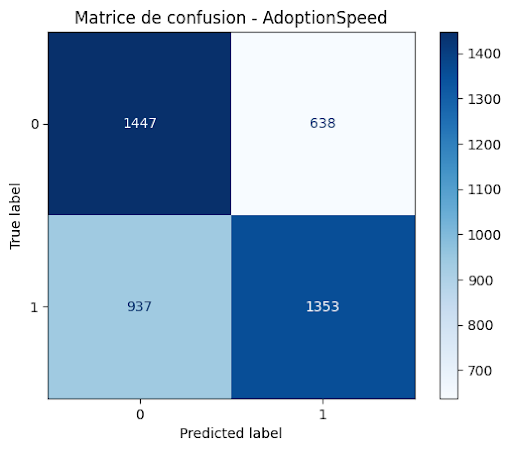
\includegraphics[width=0.7\textwidth]{matrice_confusion_sentiment_gridsearch.png}
    \caption{Matrice de confusion -- Gradient Boosting avec sentiments (optimisé)}
    \label{fig:matrice_confusion_sentiment_gridsearch}
\end{figure}

La matrice de confusion montre :
\begin{itemize}
    \item \textbf{Classe 0} : 1447 exemples bien classés, 638 confondus avec la classe 1
    \item \textbf{Classe 1} : 1353 bien classés, 937 mal prédits
\end{itemize}

Globalement, la \textbf{précision atteint 67.96\,\%}, mais le \textbf{rappel global diminue à 59.08\,\%}, traduisant une meilleure confiance dans les prédictions, mais au prix d’un taux d’erreurs de rappel plus élevé.

\vspace{0.5em}
\textbf{Conclusion :} comparé au modèle sans GridSearchCV, on note une légère amélioration de la précision globale, mais une baisse du rappel, suggérant que le modèle devient plus conservateur dans ses prédictions.

\end{document}
